\documentclass[11pt]{article}
\usepackage{amssymb,amsfonts,amsmath,cite,enumerate,float}
\usepackage[dvips]{graphicx}
\graphicspath{{images/}}

\begin{document}

\title{Project 8: Slow Dynamics and High Variability in Networks with Clustered Connections}
\author{Kirill Shchegelskiy and Tormod Hellen}

\maketitle

\section{Introduction}

Many real-world networks exhibit nonuniform connectivity structures, often including clustering of connections between different units. For instance, anatomical studies demonstrate that excitatory connections in cortex are not uniformly distributed, but the neurons are clustered into groups of highly connected neurons. However, most of network simulations use simple uniform connection structures and thus lack the architecture complexity.

In this project we after the Litwin-Kumar and Doiron (2012) studied the effect of clustered excitatory connections on the dynamics of neuronal networks. As it was demonstrated before, our results show that even small perturbations from homogeneously connected structures can substantially change network dynamics. 

\section{Results}

Our network consisted of 4,000 excitatory (E) and 1,000 inhibitory (I) model neurons. Neurons were modeled as leaky integrate-and-fire units whose voltages obey 

$$
\dot{V} = \frac{1}{\tau}(\mu - V) + I_{syn}
$$

When neurons reach a threshold $V_{th} = 1$, they spike and then reset to $V_{re} = 0$ for an absolute refractory period of 5 ms. The bias $\mu$ was chosen randomly from a uniform random distribution between 1.1 and 1.2 for excitatory neurons and between 1 and 1.05 for inhibitory neurons. The membrane time constant $\tau$ was 15 ms for excitatory and 10 ms for inhibitory neurons.

Connections involving inhibitory neurons were nonspecific, randomly distributed with probability $p^{EI} = p^{IE} = p^{II} = 0.5$, where $p^{XY}$ denotes the probability of a connection from a neuron in population $Y$ to a neuron in population $X$. Connections between excitatory neurons occured with probability $p^{EE} = 0.2$.

%1. uniform network raster plot with white noise

We began by replicating the asynchronous dynamics of uniform (non-clustered) balanced networks. For the specific values of synaptic connection strength we used the numbers from Litwin-Kumar and Doiron (2012). 

\begin{figure}[h]
\center{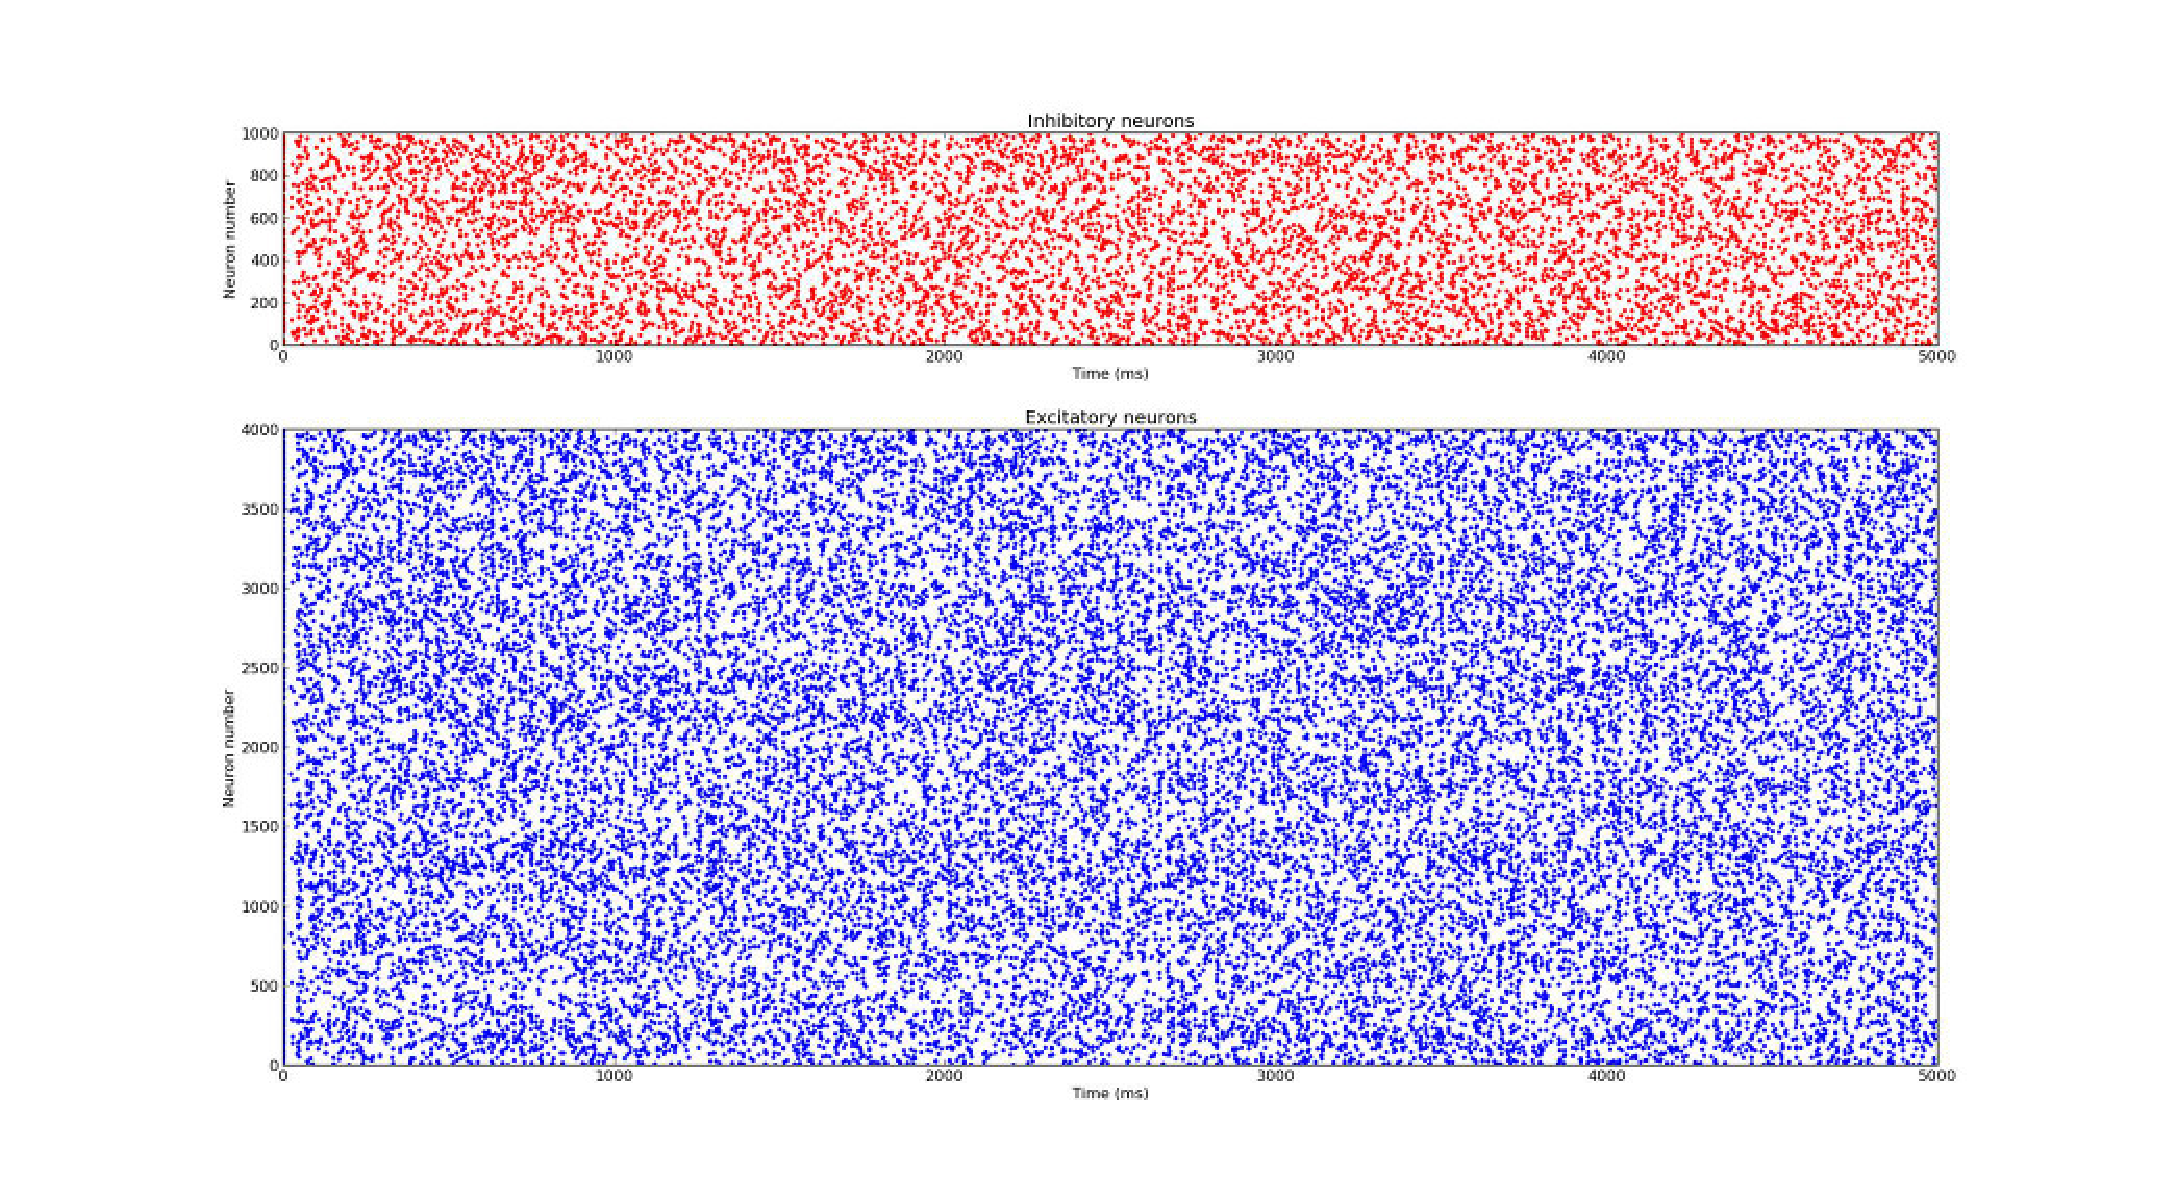
\includegraphics[width=1\linewidth]{uniform.eps}}
\caption{Uniform network raster spike plot}
\label{fig:uniform}
\end{figure}

In the figure ~\ref{fig:uniform} we can see a spike raster plot of our network with the simulation time of 5000 ms. Even from the figure itslef we can see that the behaviour is highly asynchronous and can be described as a "white noise". 

%2. clustered network raster plot

We next introduced clustered excitatory connections. The excitatory population was divided into clusters of 80 neurons each, and the connection probability $p^{EE}$ was set to $p_{in}^{EE}$ for neurons in the same cluster or $p_{out}^{EE}$ for neurons in different clusters. The ratio $R^{EE} = \frac{p_{in}^{EE}}{p_{out}^{EE}}$ controlled neuronal clustering. The higher is the value of $R^{EE}$, the stronger are the connections within clusters compared to the ones outside. The exact values of $p_{in}^{EE}$ and $p_{out}^{EE}$ were chosen so that the connection probability between excitatory neurons remained 0.2 on average. The synaptic strength for neurons in the same cluster was also increased. 

\begin{figure}[h]
\center{\includegraphics[width=0.9\linewidth]{clustered.eps}}
\caption{Clustered network raster spike plot}
\label{fig:clustered}
\end{figure}

In the figure ~\ref{fig:clustered} we can see a spike raster plot of our network with the simulation time of 5000 ms and the clustering ratio value $R^{EE} = 2.5$. This behaviour is quite distinct from the one observed in the figure ~\ref{fig:uniform}, here neurons clearly exhibit dynamic transitions between periods of higher and lower firing rate, what reflects changes in the average firing rate of neurons in the same cluster, at the same time demonstrating the randomness in the spike times of any individual neuron. Thus, even a small change in the architecture can yield substantial changes in overall network dynamics.

%3. fano factors for uniform and clustered networks

For quantative comparison of the behaviour of clustered and unifrom networks we used the Fano factor; it is defined as

$$
F_i(t, t+\Delta t) = \frac{Var(N_i(t, t+\Delta t))}{<N_i(t, t+\Delta t)>}
$$

where the expectations are over repeated trials of the same network with random initial conditions and $N_i(t, t+\Delta t)$ is the number of spikes emitted by neuron $i$ between times $t$ and $t+\Delta t$. Fano factors were computed over 100 ms window.

\begin{figure}[h]
\begin{minipage}[h]{0.49\linewidth}
\center{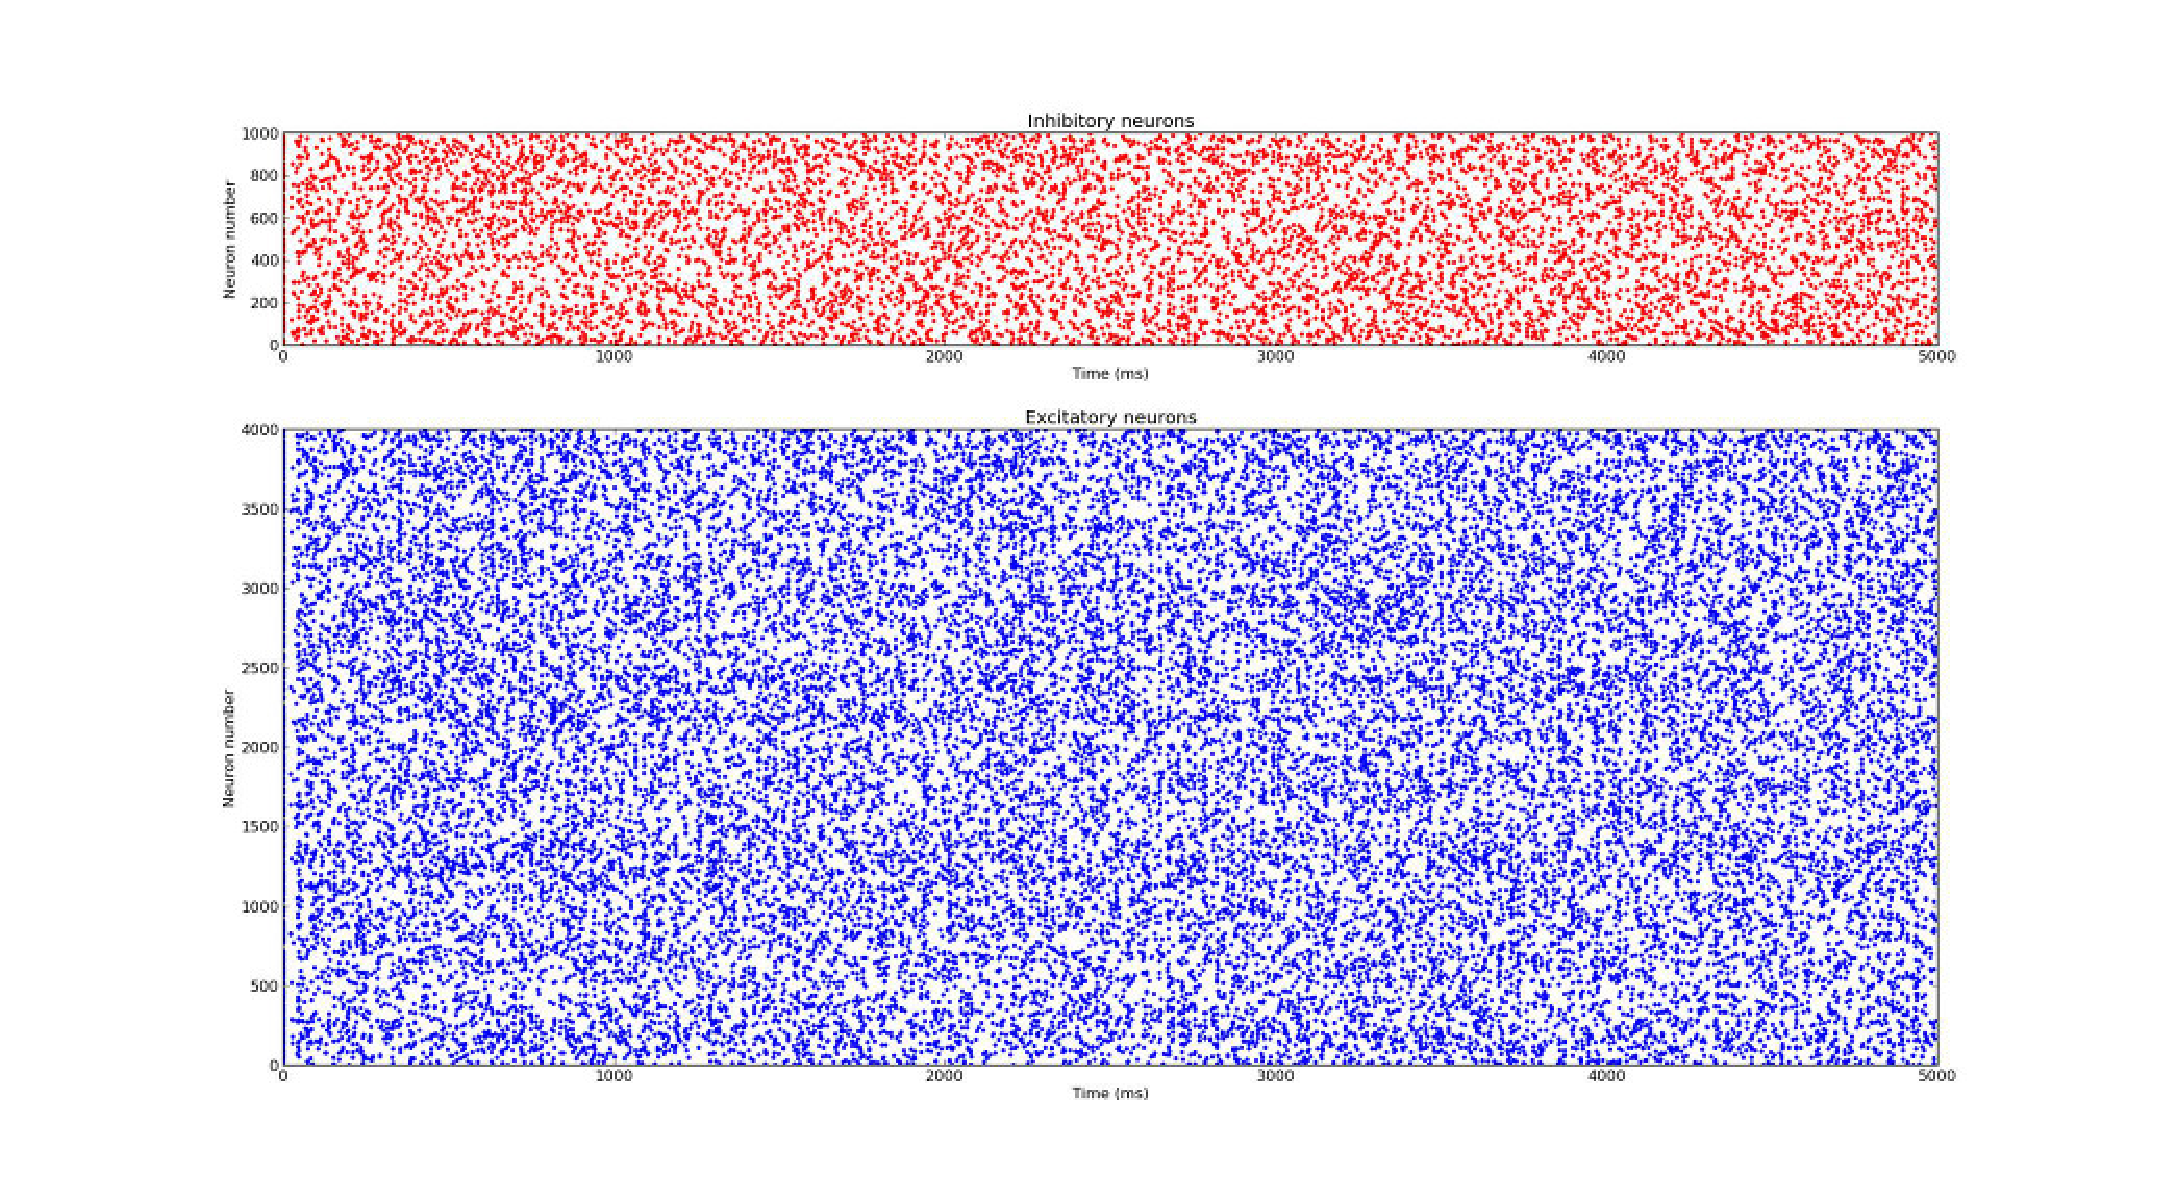
\includegraphics[width=0.5\linewidth]{uniform.eps} \\ uniform}
\end{minipage}
\hfill
\begin{minipage}[h]{0.49\linewidth}
\center{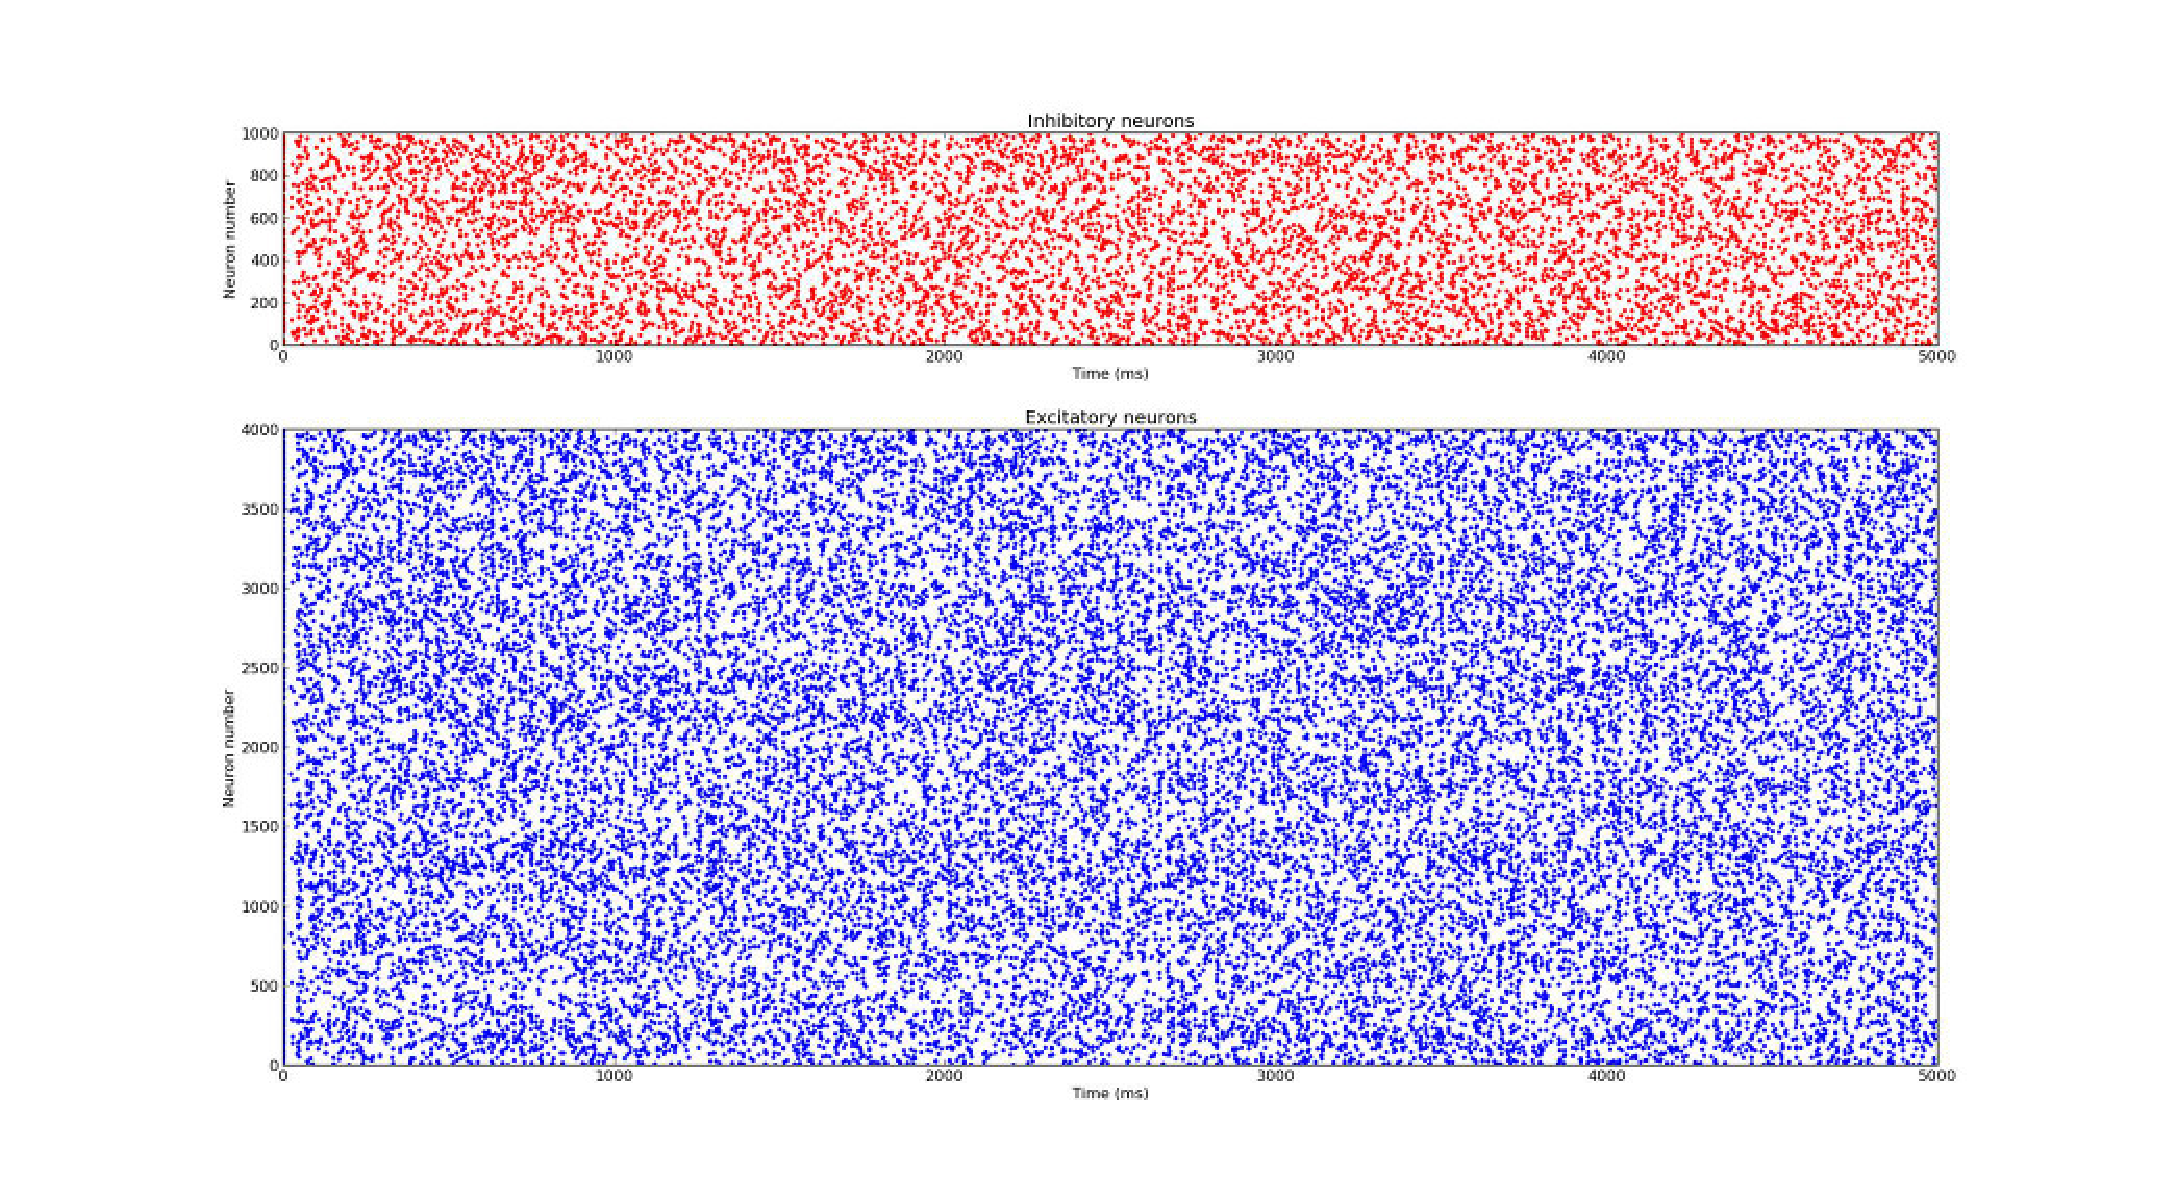
\includegraphics[width=0.5\linewidth]{uniform.eps} \\ clustered}
\end{minipage}
\caption{Histograms of excitatory neurons Fano factors}
\label{fig:hist}
\end{figure}

In the figure ~\ref{fig:hist} we can see two histograms of excitatory neuron Fano factors computed over 100 ms windows for uniform and clustered network, respectively. Although they look quite similar, the mean value of the Fano factor for the clustered network is larger than the one of the uniform network neurons. This additional variability arose from firing rate fluctuations introduced by cluster state transitions from low to high activity.


%4. raster plots for different $R^{EE}$; fano factor over $R^{EE}$
\begin{figure}[h]
\center{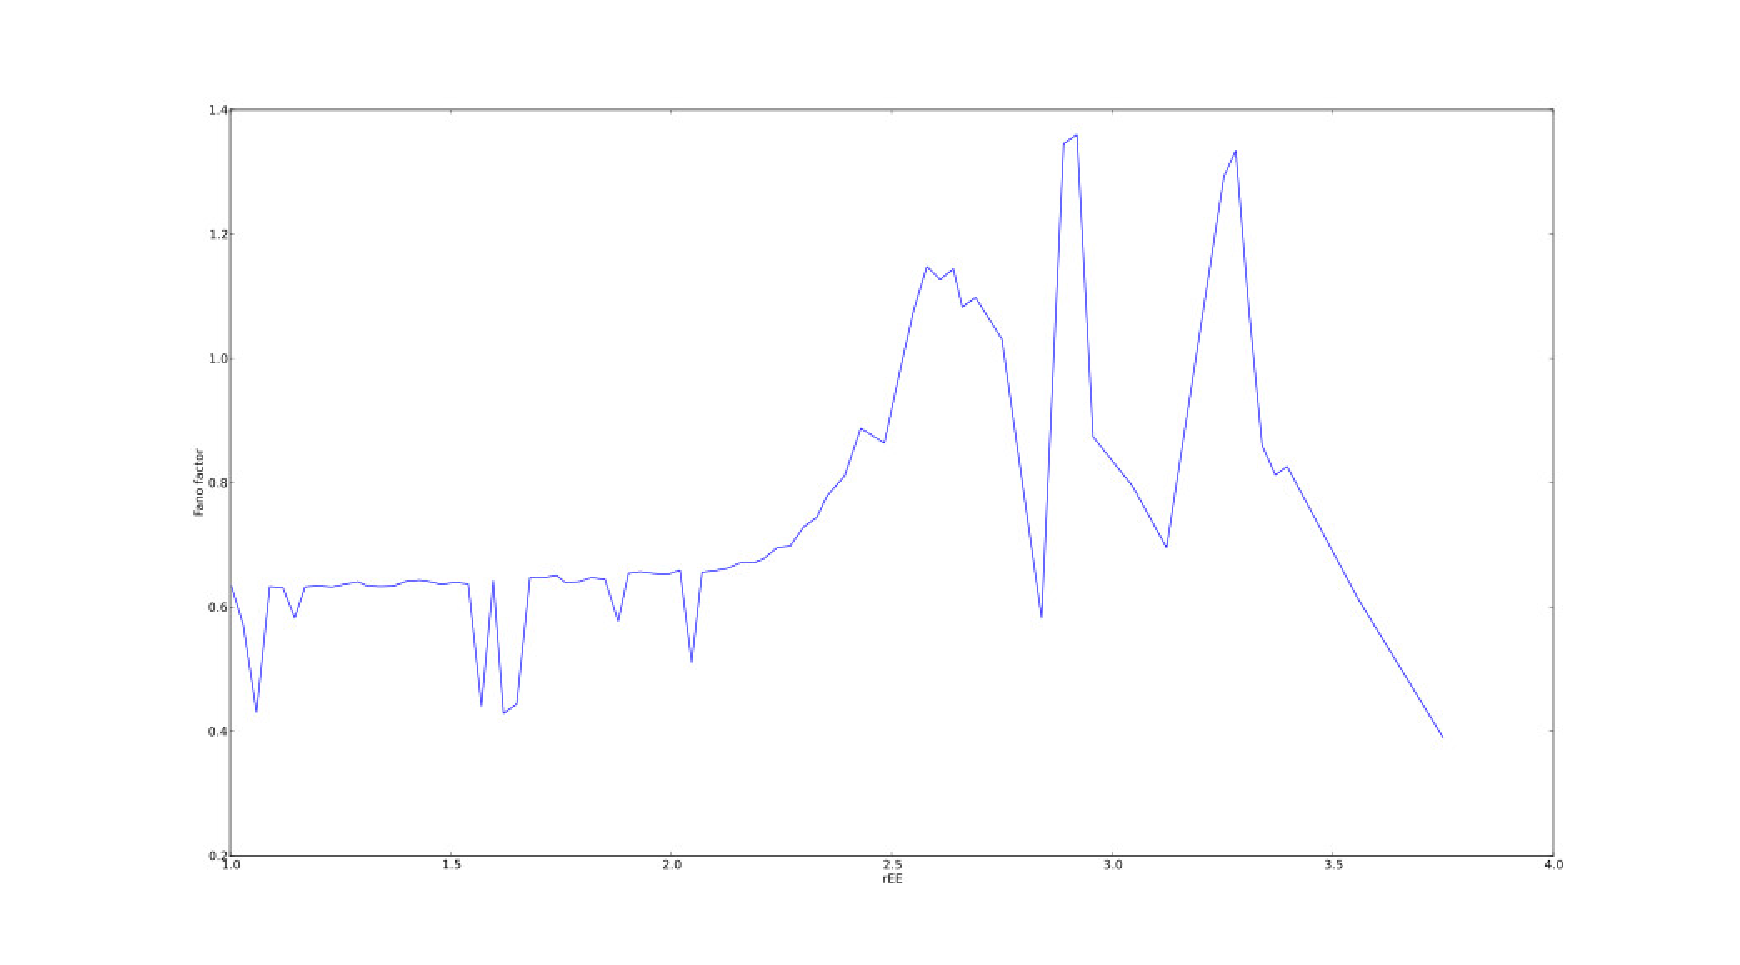
\includegraphics[width=0.9\linewidth]{FFoverRee.eps}}
\caption{Fano factor over $R^{EE}$}
\label{fig:ffoverree}
\end{figure}

In the figure ~\ref{fig:ffoverree} we can see a plot of average Fano factor among excitatory neurons computed for clustered neuronal networks with different $R^{EE}$. Although in the beginning we can see a general rise, it is followed by a decay for big values of $R^{EE}$, that is not observed in the analogous plot in the paper by Litwin-Kumar and Doiron. However, it can be expected to be so, as the increase in $R^{EE}$ leads to stronger connections within clusters and thus to the decrease in the firing rate fluctuations generated by cluster state switching from low to high activity and vice versa.



\section{Discussion}

We have shown that clustering of excitatory connections substantially changes balanced network dynamics. Small changes in neurons connectivity led to slow firing rate fluctuations in spontaneous conditions. These stochastic dynamics reflect large trial-to-trial variability in network responses and are not presented in simple uniform structures.

The network connectivity in this study was motivated by the anatomical evidence for clustering of connections between pyramidal neurons in cortex. The resulting dynamics of the artificial clustered network are reminiscent of persistent state activity and thus are closer to experimental data than the uniform ones.

Our parameter and model choices were based on the Litwin-Kumar and Doiron (2012) and our results were quite close to the ones demonstrated in the referred article. The critical value for $R^{EE}$ (neuronal clustering control value) was around $2.5$, and that is very close to the result demonstrated by Litwin-Kumar and Doiron. The dynamics of the Fano factor over different values of $R^{EE}$ were a bit different from the ones presented in the referred paper, but generally the results match in a satisfactory way.



\end{document}